%	This LaTeX file is written by Zhiyang Ong as a template for inserting figures in LaTeX.

%	The MIT License (MIT)

%	Copyright (c) <2014> <Zhiyang Ong>

%	Permission is hereby granted, free of charge, to any person obtaining a copy of this software and associated documentation files (the "Software"), to deal in the Software without restriction, including without limitation the rights to use, copy, modify, merge, publish, distribute, sublicense, and/or sell copies of the Software, and to permit persons to whom the Software is furnished to do so, subject to the following conditions:

%	The above copyright notice and this permission notice shall be included in all copies or substantial portions of the Software.

%	THE SOFTWARE IS PROVIDED "AS IS", WITHOUT WARRANTY OF ANY KIND, EXPRESS OR IMPLIED, INCLUDING BUT NOT LIMITED TO THE WARRANTIES OF MERCHANTABILITY, FITNESS FOR A PARTICULAR PURPOSE AND NONINFRINGEMENT. IN NO EVENT SHALL THE AUTHORS OR COPYRIGHT HOLDERS BE LIABLE FOR ANY CLAIM, DAMAGES OR OTHER LIABILITY, WHETHER IN AN ACTION OF CONTRACT, TORT OR OTHERWISE, ARISING FROM, OUT OF OR IN CONNECTION WITH THE SOFTWARE OR THE USE OR OTHER DEALINGS IN THE SOFTWARE.

%	Email address: echo "cukj -wb- 23wU4X5M589 TROJANS cqkH wiuz2y 0f Mw Stanford" | awk '{ sub("23wU4X5M589","F.d_c_b. ") sub("Stanford","d0mA1n"); print $5, $2, $8; for (i=1; i<=1; i++) print "6\b"; print $9, $7, $6 }' | sed y/kqcbuHwM62z/gnotrzadqmC/ | tr 'q' ' ' | tr -d [:cntrl:] | tr -d 'ir' | tr y "\n"

%%%%%%%%%%%%%%%%%%%%%%%%%%%%%%%%%%%%%%%%%%%%%%



%%%%%%%%%%%%%%%%%%%%%%%%%%%%%%%%%%%%%%%%%%%
\chapter{Figures}
\label{chp:Figures}

A template for inserting figures is shown in Figures \ref{fig:MyFigure1}, \ref{fig:MyFigure2}, \ref{fig:MyFigure3}, and \ref{fig:MyFigure4}. Also, a TikZ figure is shown in Figure \ref{tikz:MyPolarPlot}.

\begin{figure}[h]
\centering 

\includegraphics[height=1.5in]{./pics/short}
\caption{Caption for my figure1}
\label{fig:MyFigure1}
\end{figure}

\begin{figure}[h]
\centering 

\includegraphics[height=1.5in]{./pics/small}
\caption{Caption for my figure2}
\label{fig:MyFigure2}
\end{figure}

%	Clear the remanding part of the page, and insert the remaining figures and text in subsequent pages.
\clearpage

\begin{figure}[h]
\centering 
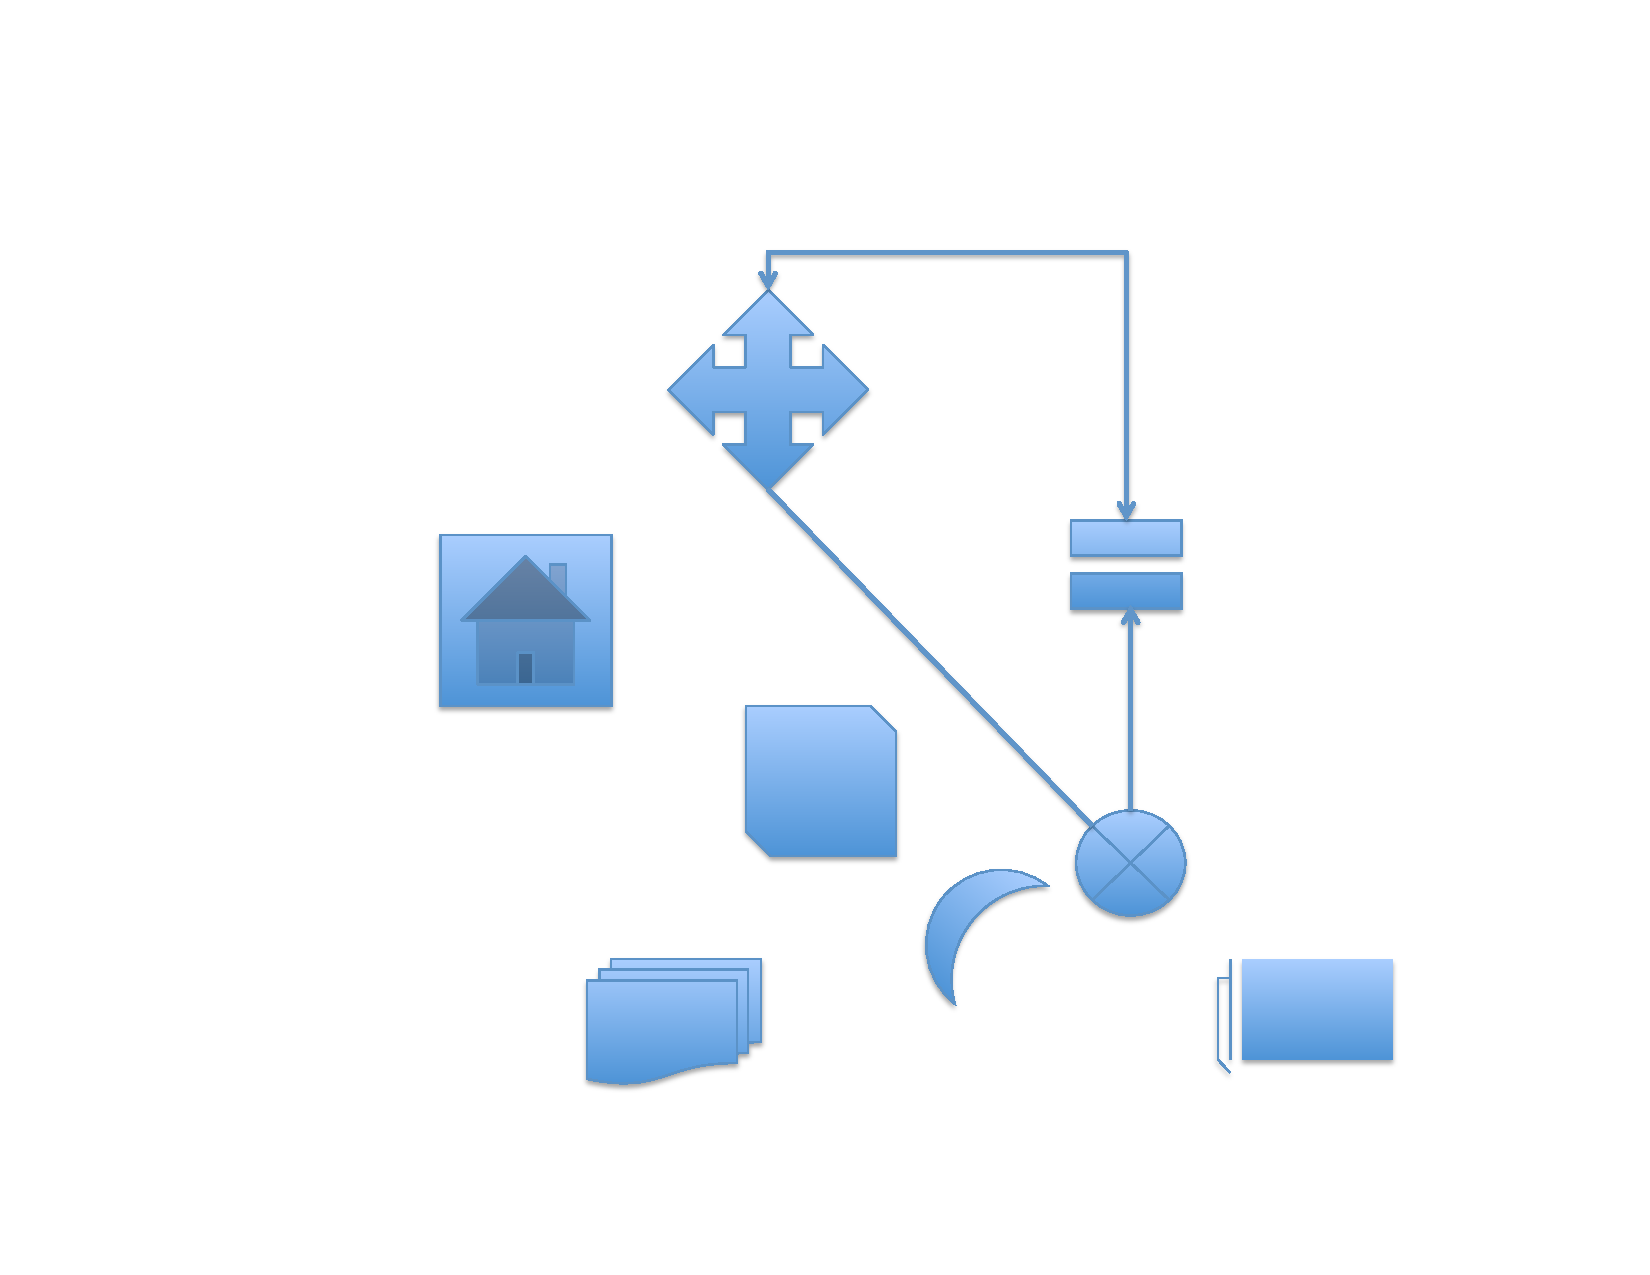
\includegraphics[width=6in]{./pics/my_figure}
\caption{Caption for my figure3}
\label{fig:MyFigure3}
\end{figure}



\begin{figure}
\centering 
	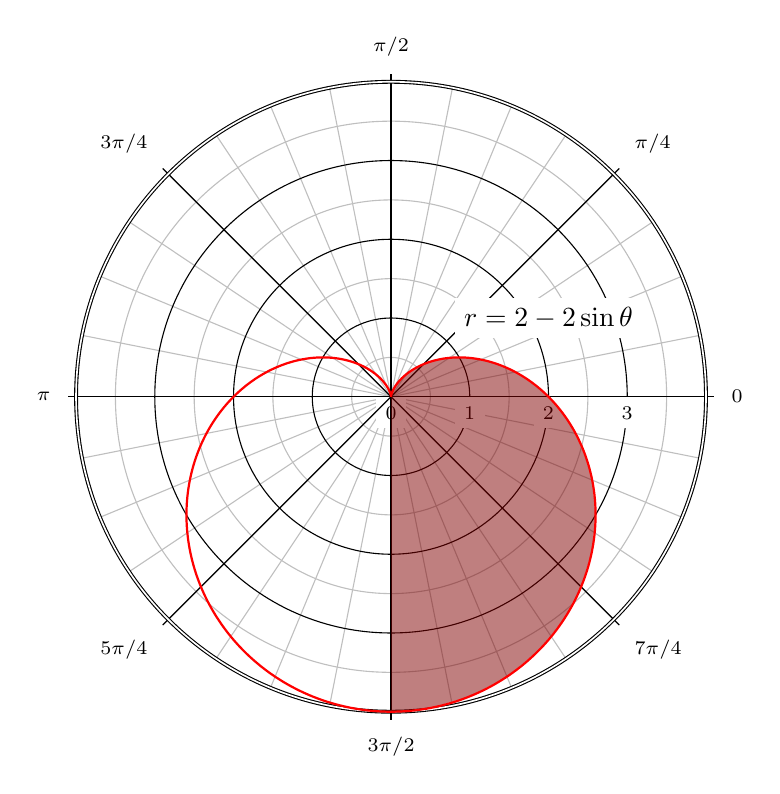
\begin{tikzpicture}[>=latex]
		% Draw the lines at multiples of pi/12
		\foreach \ang in {0,...,31} {
			\draw [lightgray] (0,0) -- (\ang * 180 / 16:4);
		}
		
		% Concentric circles and radius labels
		\foreach \s in {0, 1, 2, 3} {
			\draw [lightgray] (0,0) circle (\s + 0.5);
			\draw (0,0) circle (\s);
			\node [fill=white] at (\s, 0) [below] {\scriptsize $\s$};
		}
		
		% Add the labels at multiples of pi/4
		\foreach \ang/\lab/\dir in {
			0/0/right,
			1/{\pi/4}/{above right},
			2/{\pi/2}/above,
			3/{3\pi/4}/{above left},
			4/{\pi}/left,
			5/{5\pi/4}/{below left},
			7/{7\pi/4}/{below right},
			6/{3\pi/2}/below} {
			\draw (0,0) -- (\ang * 180 / 4:4.1);
			\node [fill=white] at (\ang * 180 / 4:4.2) [\dir] {\scriptsize $\lab$};
		}
		
		% The double-lined circle around the whole diagram
		\draw [style=double] (0,0) circle (4);
		
		\fill [fill=red!50!black, opacity=0.5] plot [domain=-pi/2:pi/2]
			(xy polar cs:angle=\x r, radius= {2-2*sin(\x r)});
		\draw [thick, color=red, domain=0:2*pi, samples=200, smooth]
			plot (xy polar cs:angle=\x r, radius={2-2*sin(\x r)});
		\node [fill=white] at (2,1) {$r=2-2\sin\theta$};
	\end{tikzpicture}
\caption{My polar plot}
\label{tikz:MyPolarPlot}
\end{figure}



\begin{figure}[h]
\centering 
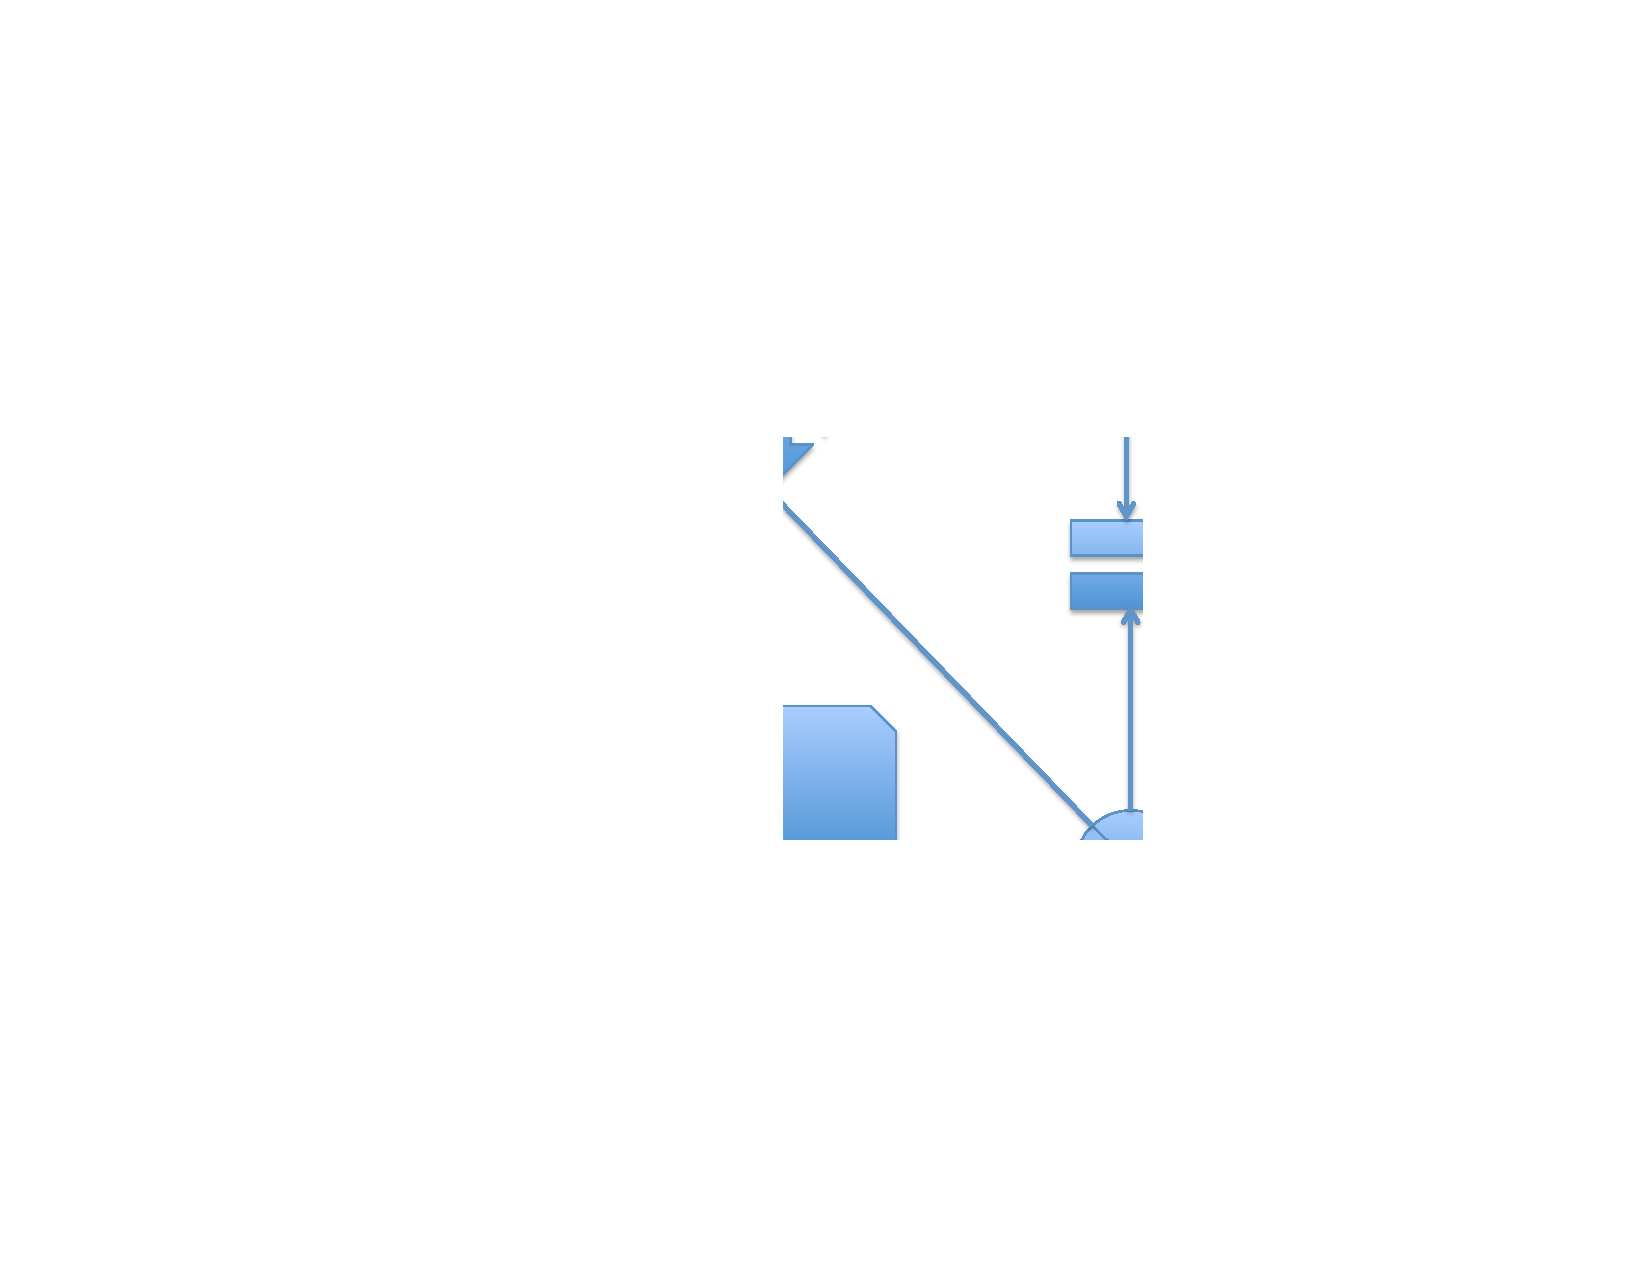
\includegraphics[height=1.5in]{./pics/trim}
\caption{Caption for my figure4}
\label{fig:MyFigure4}
\end{figure}














